\chapter{Desenvolvimento do Projeto}

Neste capítulo é abordado tudo o que foi necessário para chegar em um projeto viável, como tecnologias utilizadas, arquitetura do sistema, viabilidade financeira, critérios necessários para segurança da aplicação, casos de uso e regrás de negócio como também métricas para dimensionar dificuldades, qualidade e tamanho do aplicativo.   



\section{Arquitetura do sistema}
A arquitetura foi escolhida visando a maior facilidade de armazenamento da aplicação na cloud do Heroku para que seja possível o acesso dela em lugares com os recursos básicos, como um dispositivo conectado a internet, e também para a equipe visulizar a evolução da construção da aplicação. 

O aplicativo diversaGente, como mostrado na \autoref{arquitetura-sistema}, está hospedado no Heroku onde atualmente está todo o back-end que é desenvolvido pelo framework nodeJS e pode receber requisições do banco de dados mongoDB e servidor de amazenamento de arquivos. O lado do cliente foi feito em React Native 

\begin{figure}[htb]
	\centering
	\caption{\label{fig_arq_virado}Arquitetura do sistema}
	\label{arquitetura-sistema}
	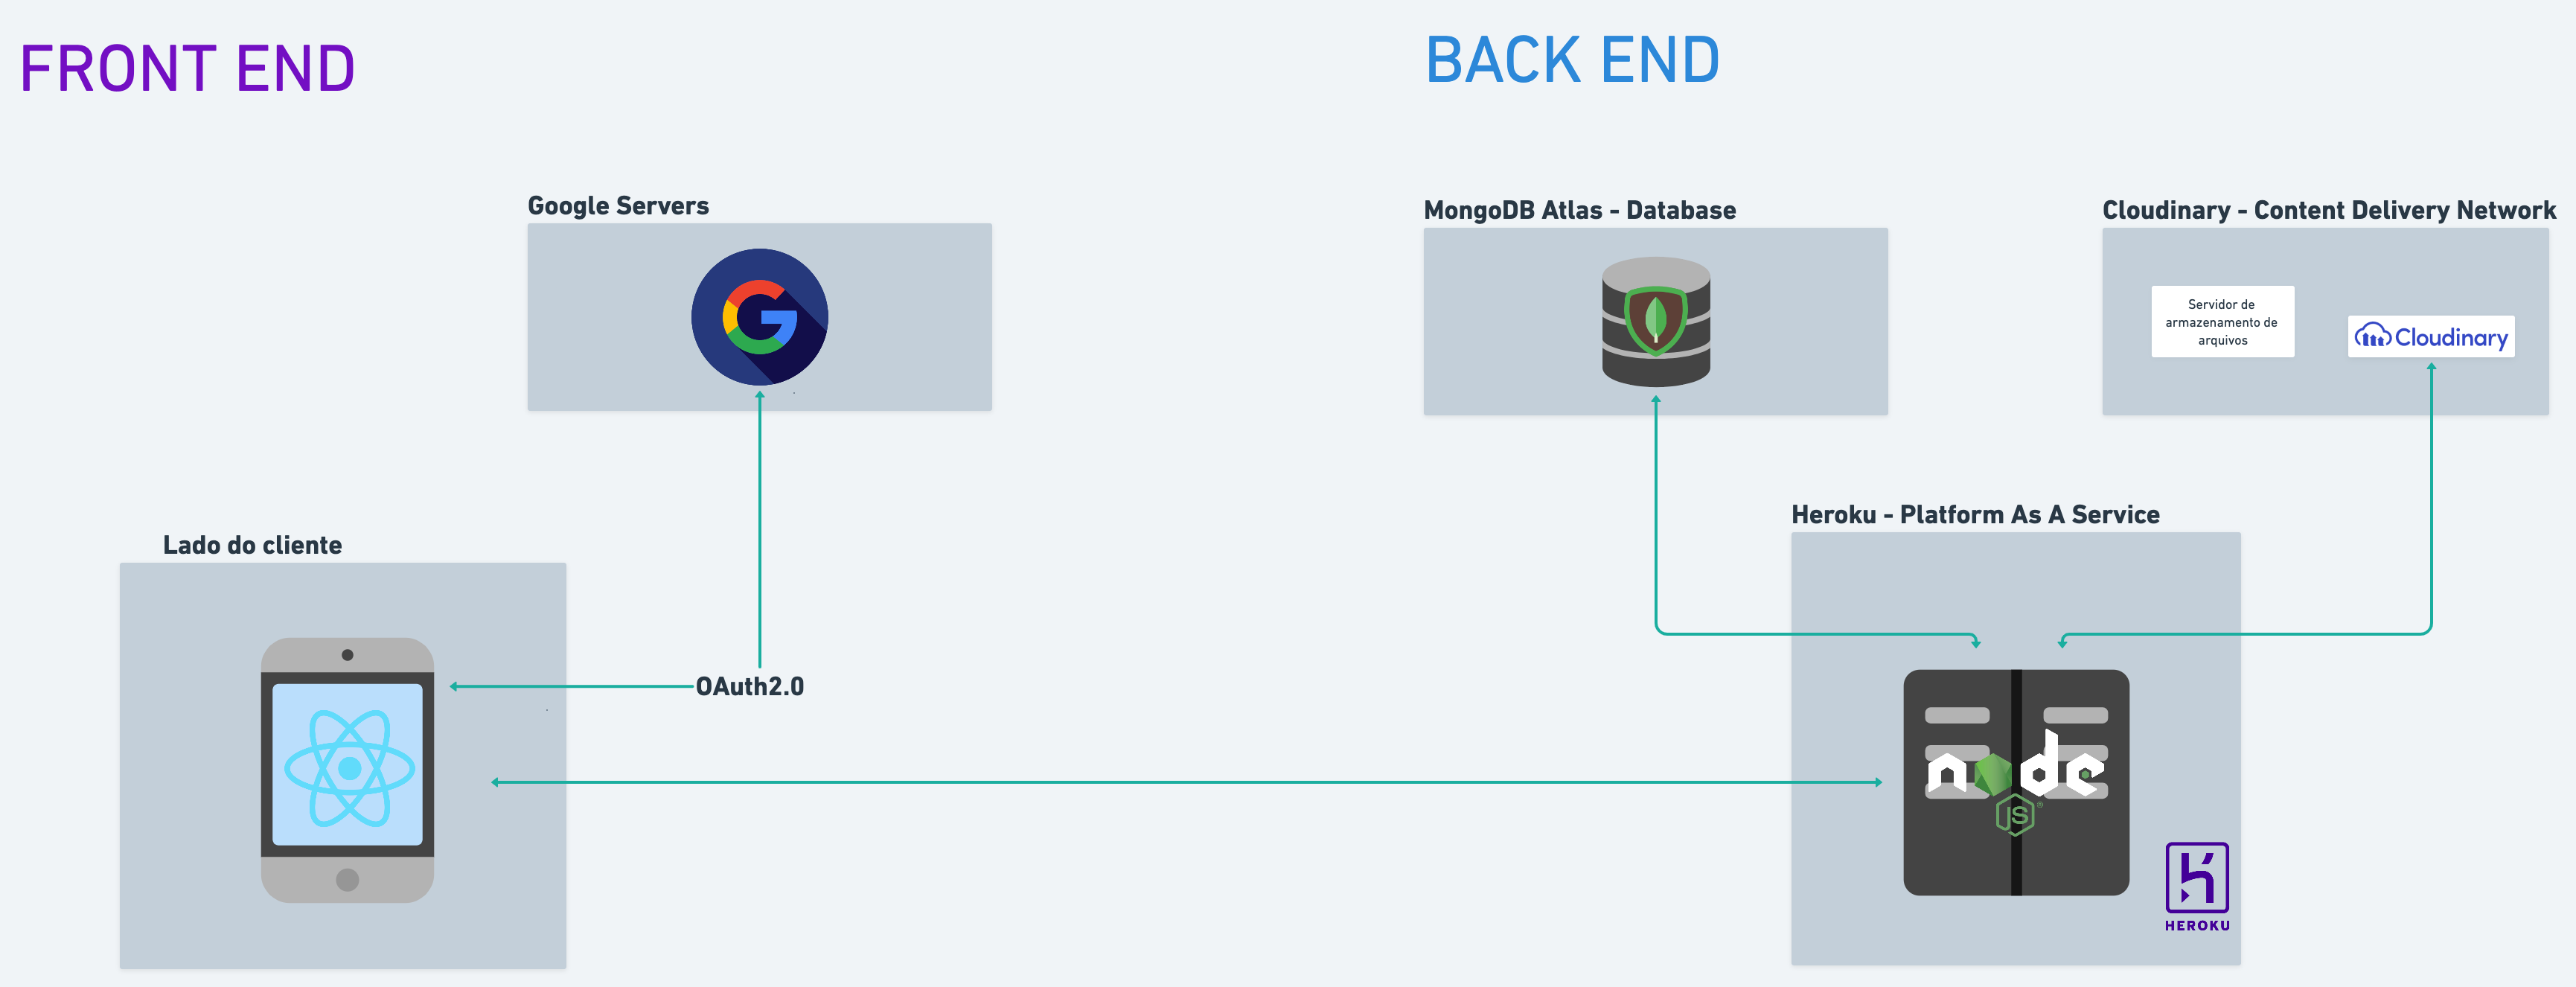
\includegraphics[width=0.9\textwidth]{anexos/poc-arquitetura.png}
	\fonte{Equipe diversaGente (2022)}
\end{figure}


\section{Tecnologias utilizadas}

Para o lado do cliente, a escolha foi o React Native com Typescript junto a ferramenta Expo para testar o app com as APIs nativas do Android que essa ferramenta disponibiliza.

Já para o lado do servidor, as ferramentas são o Node.js com Typescript e framework NestJS para a construção da API, MongoDB como banco de dados, Prisma como ORM, Cloudinary como storage e para documentação de API, a especificação OpenAPI.

Para o ambiente de desenvolvimento, a escolha foi o Docker, a fim de obter facilidade em executar o projeto independente do Sistema Operacional local.

A hospedagem é feita por meio da Play Store para o app em React Native, do Heroku para o backend em Node.js e do MongoDB Atlas para o banco de dados, e todo o versionamento feito por meio das plataformas Github e Subversion.

Para realizar a prototipação das interfaces, a opção utilizada é a ferramenta Figma e a construção de fluxos e brainstorms da equipe se dão por meio do Miro e Whimsical.

Por fim, para o gerenciamento do projeto, a escolha foi o Trello para registro de backlog e acompanhamento do status de desenvolvimento das histórias, o Discord para realização das cerimônias semanais da equipe e o WhatsApp para comunicações rápidas e mais urgentes entre o time.

\section{Escalabilidade}

O quesito ‘escalabilidade’ é muito abordado e de extrema importância atualmente, principalmente devido ao enorme fluxo de dados que corre dentre os sistemas e aplicações. A escalabilidade diz respeito a facilidade de crescimento da infraestrutura da aplicação de forma saudável, sem grandes impactos nos custos ferramentais e humanos e no desempenho da aplicação. Essa adaptabilidade pode estar relacionada com a implementação de novas funcionalidades, novas demandas de mercado, inserção em requisições legislativas e projetos de inovação, por exemplo. 

O projeto conta com ferramentas muito atuais, que já trazem consigo muito fortemente o conceito de escalabilidade, como o Heroku e o Docker, o primeiro que ganha cada vez mais espaço de mercado como uma Platform as a Service (PaaS), em que a solução permite que o desenvolvedor tenha maiores facilidades com detalhes estruturais, trazendo maior facilidade de manutenção e maior agilidade de implantação, já o segundo possibilita a criação de ambientes virtuais completos, os chamados contêineres, que podem até mesmo ter seu crescimento automatizado de acordo com a demanda de requisições, gerando novos contêineres semelhantes, por exemplo. 

Por se tratar de um modelo de aplicação com pouca concorrência em mercado, existem chances relevantes de crescimento, assim, é possível que haja a necessidade de escalada da aplicação em um futuro breve, tendo isso em consideração, as ferramentas anteriormente citadas se encaixam muito bem nessa possível necessidade futura. 



\section{Manutenibilidade, Integração Contínua e Testes}
A manutenibilidade é o que garante a qualidade do software para manutenções futuras, como corrigir erros que podem ocorrer, melhora de performance, adequar a novas práticas de mercade ou necessidade de conexão com outras aplicações. Sendo assim, utilizando as boas práticas do mercado, convenções, aplicando uma padronização e um código limpo a aplicação consegue ter uma alta manutenibilidade para quaisquer futuras adaptações.  

A integração das diversas versões de código gerado durante o desenvolvimento da aplicação foi feita através do GitHub, divididos em diversas branchs de features e para cada pessoa desenvolvedora da equipe que solicita para uma pessoa responsável pela manutenibilidade aprovar as alterações e realizar o merge com a branch principal que reflete no ambiente de produção, é possível manter os ambientes atualizados para desenvolvimento.

Para subir as alterações para o produção e conseguir fazer a visualização, foi utilizado o workflow de Continuous Integration que é gerado através do GitHub Actions

Para os testes unitários da aplicação, o Jest, um framework JavaScript para testes automatizados, e ESLint para análise estática do código.
O sistema de Log de toda aplicação Papertrail é o sistema de log escolhido para mapear o comportamento da API em Node.js.
%\pagebreak

\section{Diagramas do sistema}

Nesta seção possui todos os diagramas criados do sistema, para facilitar o entendimento e desenvolvimento da aplicação. 

O diagrama de casos de uso apresentado na \autoref{diagrama-caso-uso} representa uma possível utilização do nosso sistema por ator, sejá ele o usuário ou administrador.

\pagebreak

\begin{figure}[htb]
	\centering
	\caption{\label{fig_arq_virado}Diagrama de classes do sistema}
	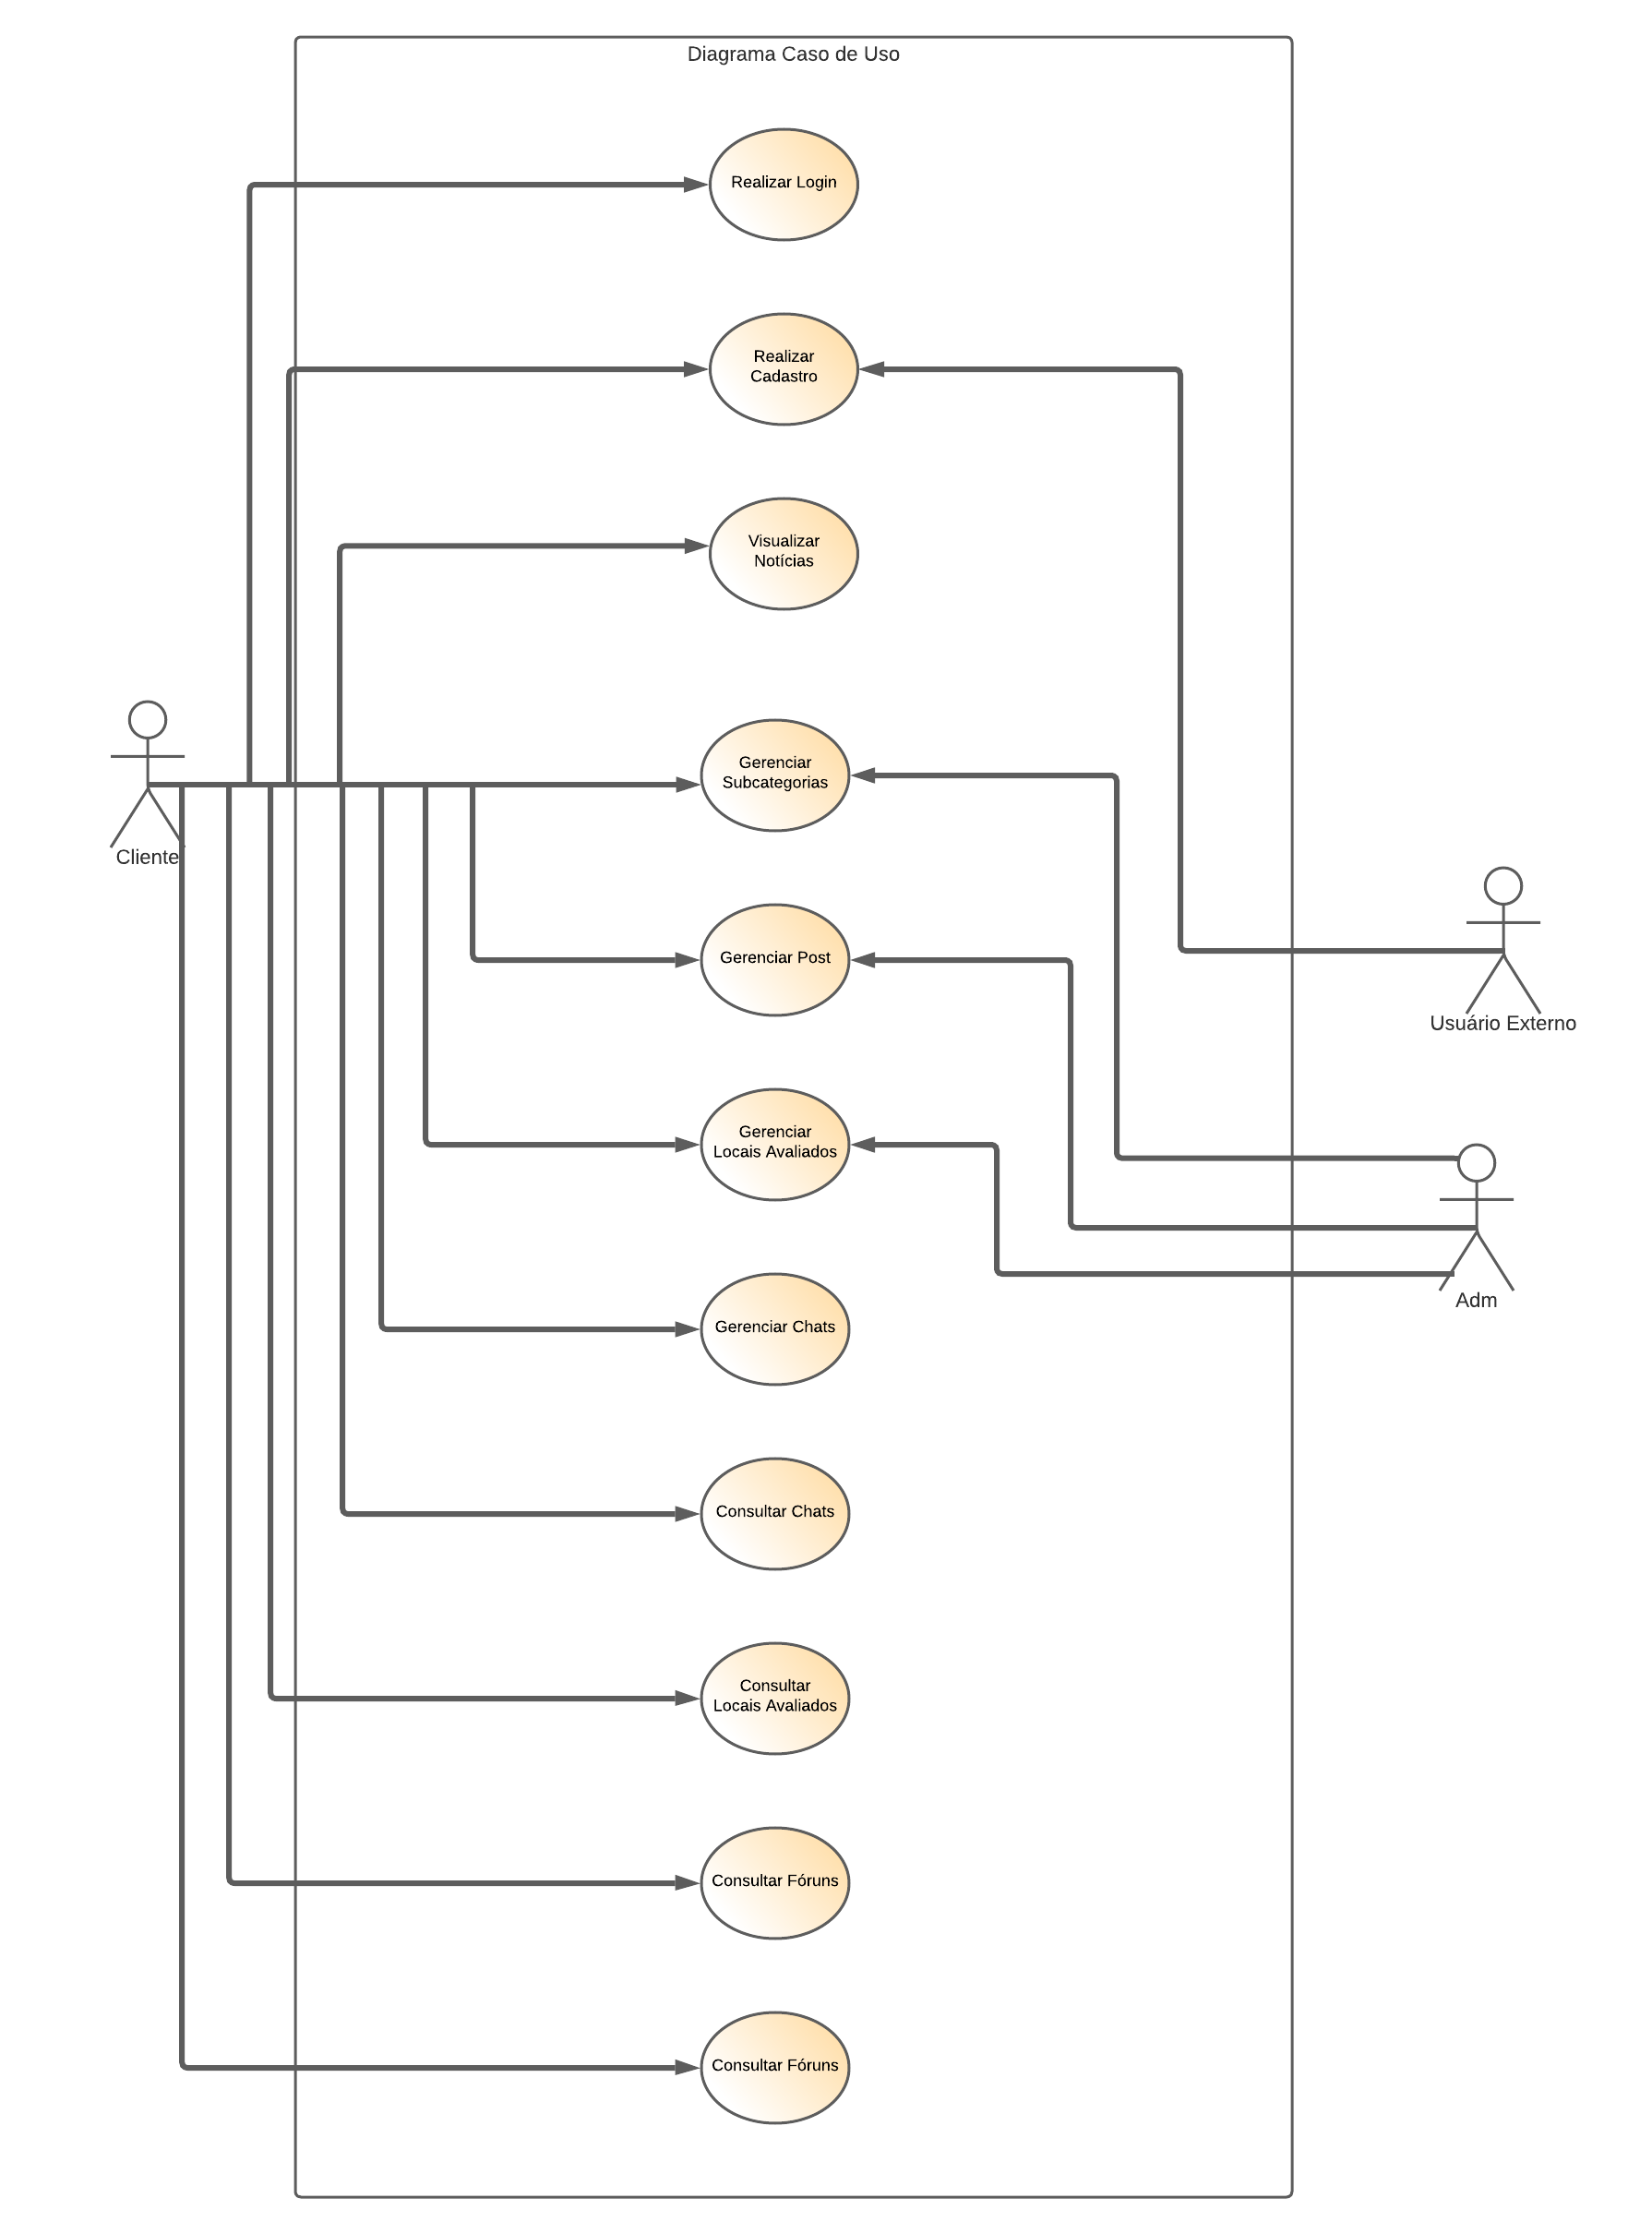
\includegraphics[width=0.90\textwidth]{anexos/Diagrama_em_branco.png}
	\label{diagrama-caso-uso}
	\fonte{Equipe diversaGente (2022)}
\end{figure}


As especificações de casos de uso informam através de texto a utilização do usuário ou administrador dentro da aplicação. São identificadas através de códigos que se iniciam com UC, indo do
UC01 \autoref{casos-de-uso1} até o UC21 do \autoref{casos-de-uso21}. Os textos podem ser encontrados no \autoref{casos-de-uso-especificacao}

No diagrama de classe,  \autoref{diagrama-classe}, a classe User é a principal e representa o usuário que está atrelado a grande parte das outras classes, já que o objetivo principal é ser um fórum para postagem e compartilhamento de informações. 


\begin{figure}[htb]
	\centering
	\caption{\label{fig_arq_virado}Diagrama de classes do sistema}
	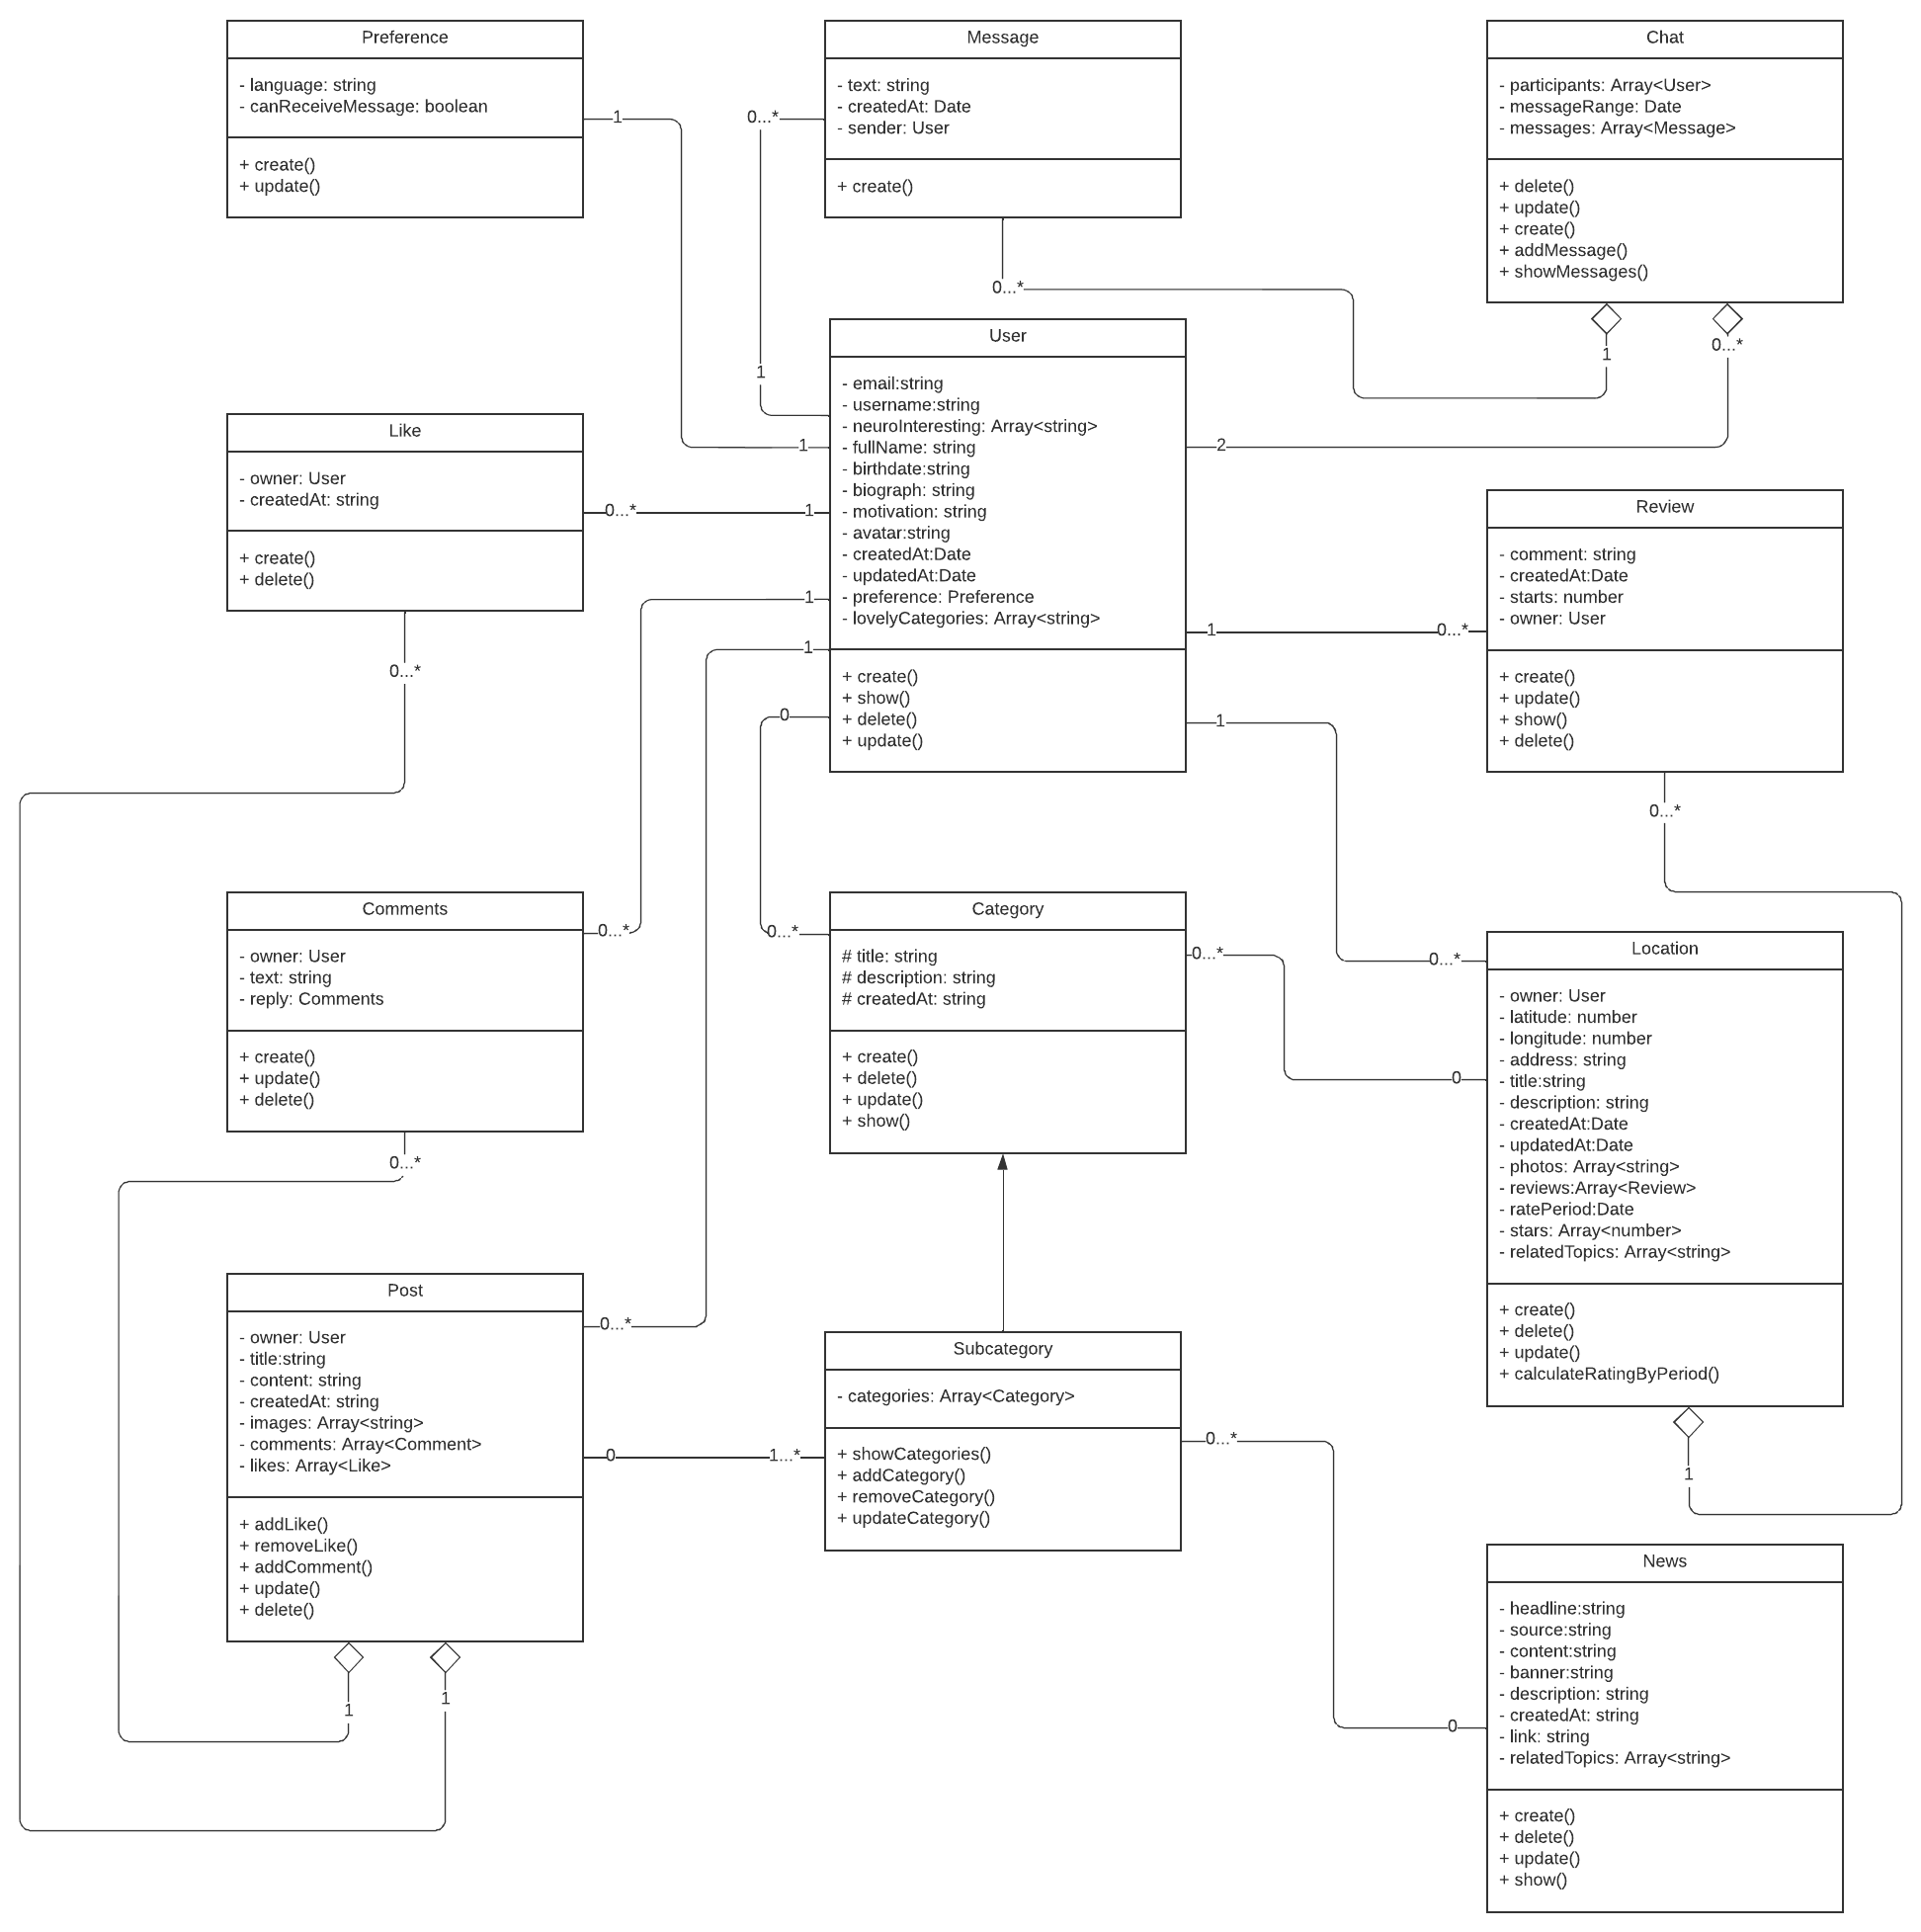
\includegraphics[width=0.90\textwidth]{anexos/diversaGente_-_Classe_UML_1.png}
	\label{diagrama-classe}
	\fonte{Equipe diversaGente (2022)}
\end{figure}

%---------------------------------------------------------------------------------------
\section{Requisitos Funcionais, Não Funcionais e Regras de Negócios}


A análise de requisitos do aplicativo está relacionada com as funcionalidades do sistema e com as prioridades diretamente ligadas a ele. Abaixo, eles estão divididos com suas respectivas funções que englobam tantos os requisitos funcionais, ou seja, declaração dos comportamentos que o sistema deve ter e os requisitos não funcionais que são as restrições colocadas sobre como o sistema deve realizar seus requisitos.

O  \autoref{tabela-requisitos-funcionais} mostra os requisitos funcionais  enquanto a \autoref{requisitos-nao-funcionais} mostra os requisitos não funcionais. 

Para as regras de negócio, \autoref{regra-negocio}, são úteis para definir como as ações vão agir em relação aos processsos da aplicação. 



\begin{quadro}[htb]
	\centering
	\ABNTEXfontereduzida
	\caption[Requisitos Funcionais]{Requisitos Funcionais}
	\label{tabela-requisitos-funcionais}
\end{quadro}
\begin{longtable}{|p{2.0cm}|p{6.5cm}|p{6.5cm}|}
	\hline
	\thead{Código} & \thead{Requisito}  & \thead{Descrição} \\
	\hline
	RF01 &Visualizar notícias.  & O usuário deve conseguir visualizar as notícias dentro da aba news, imagens, títulos e início do texto que estão associados a notícia.\\
	\hline
	RF02 & Gerenciar subcategorias. &
	O usuário consegue criar uma nova subcategoria dentro de uma categoria.
	O usuário que criou a subcategoria consegue editar o título das categorias criadas.
	O usuário consegue excluir a categoria que foi criada, recebendo um aviso se realmente é aquilo que ele deseja fazer.
	\\
	\hline
	RF03 & Gerenciar publicações.   & O usuário consegue criar uma nova publicação em uma subcategoria. 
	O usuário consegue editar uma nova publicação dentro de uma subcategoria. 
	O usuário consegue excluir uma publicação dentro de uma subcategoria\\
	\hline
	RF04 & Publicar comentários dentro das subcategorias de discussões dos fóruns criados. & O usuário consegue comentar em cada publicação. O usuário consegue excluir o comentário em cada publicação. \\
	\hline
	RF05 & Compartilhar imagem dentro das publicações de subcategorias dos fóruns criados &
	O usuário consegue compartilhar as imagens em cada publicação. O usuário consegue excluir as imagens compartilhadas em cada publicação.\\
	\hline
	RF06 & Compartilhar nos aplicativos compatíveis as notícias e os postagens das subcategorias de discussões dos fóruns criados.  & O usuário deve conseguir compartilhar as noti1cias e postagens com os aplicativos compatíveis.\\
	\hline
	RF07 & Favoritar mensagens dentro das subcategorias de discussões dos fóruns criados. & O usuário deve conseguir favoritar as mensagens. \\
	\hline
	RF08 & Gerenciar Locais Avaliados. & O usuário deve conseguir cadastrar, editar e excluir um local. O usuário deve conseguir filtrar locais mais próximos do local que se encontra ou de um endereço desejado. \\
	\hline
	RF09 & Consultar Chats.   &O usuário deve conseguir trocar mensagens instantâneas entre outro usuário.\\
	\hline
	RF10 &Receber notificações de mensagens novas. &
	O usuário deve receber uma notificação no aparelho quando receber novas mensagens do chat, mostrando quem mandou a mensagem.\\
	\hline
	RF11 & Filtrar conversas privadas do próprio usuário.  & O usuário deve conseguir pesquisar pelo nome do usuário dentro da aba conversar.\\
	\hline
	RF12 & Permitir que o usuário se cadastre na plataforma. & O usuário deve conseguir criar um cadastro através de login social do google.\\
	\hline
	RF13 & Gerenciar Perfil.  &
	O usuário deve conseguiralterar os seus dados através de uma página de perfil.  \\
	\hline
	RF14 & Permitir que usuário bloqueie o recebimento de novas mensagens.  & O usuário poderá bloquear que usuários novos mandem mensagem.\\
	\hline
\end{longtable}
\fonte{Equipe diversaGente (2022)}

\begin{quadro}[htb]
	\centering
	\ABNTEXfontereduzida
	\caption[Requisitos Não Funcionais]{Requisitos Não Funcionais}
	\label{requisitos-nao-funcionais}
	\begin{tabular}{|p{2.0cm}|p{6.5cm}|p{6.5cm}|}
		\hline
		\thead{Código} & \thead{Categoria}  & \thead{Requisito} \\
		\hline
		RNF01 & Compatibilidade &
		Deve ser compatível com o sistema operacional Android.\\
		\hline
		RNF02 & Disponibilidade & O sistema deve estar disponível 24 horas por dia, 7 dias por semana, com tolerância de 0,1\% de falhas. \\
		\hline
		RNF03 & Desempenho & O servidor deve responder em, no máximo, 0,4 segundos a todas as requisições recebidas. \\
		\hline
		RNF04 & Segurança & Para melhor análise e registro,os LOGS devem conter a data (dia, mês e ano), hora, minutos e uma breve descrição do registro.\\
		\hline
	\end{tabular}
	\fonte{Equipe diversaGente (2022)}
\end{quadro}

%--------------------------------------------------------------


\begin{quadro}[htb]
	\centering
	\ABNTEXfontereduzida
	\caption[Regras de Negócio]{Regras de Negócio}
	\label{regra-negocio}
	\begin{tabular}{|p{3.3cm}|p{10.3cm}|}
		\hline
		\thead{Código} & \thead{Regra de negócio} \\
		\hline
		RN01 & É obrigatório que o usuário tenha uma conta Google para fazer o login na plataforma. \\
		\hline
		RN02 & Somente após finalizado o cadastro contendo todas as informações obrigatórias (login social, neuro interesse e motivação) o usuário obterá acesso à plataforma.\\
		\hline
		RN03 & Caso o usuário seja o criador de uma subcategoria, será possível editá-la e excluí-la.  \\
		\hline
		RN04 & Somente o usuário que é criador de uma avaliação da seção ‘Locais Avaliados’ é capaz de editá-la ou excluí-la. \\
		\hline
		RN05 & O recebimento de mensagens requer a permissão do usuário. \\
		\hline
		RN06 & Não devem haver subcategorias com o mesmo nome. \\
		\hline
		RN07 & Deverão ser mostradas de forma ranqueada as categorias, subcategorias e posts mais relevantes.\\
		\hline
		RN08 & É obrigatório que os posts publicados contenham título e texto.\\
		\hline
		RN09 & Caso o post seja editado, deve ser explicitado.\\
		\hline
	\end{tabular}
	\fonte{Equipe diversaGente (2022)}
\end{quadro}\pagebreak

%----------------------------------------------------------
\section{Casos de Uso}
Os casos de uso apresentados neste capítulos representam uma possível utilização do nosso sistema por ator, seja ele o usuário ou administrador. Pode sem visto através de um diagrama de casos de uso no \autorefwithpage{diagrama-caso-uso} tanto em quadros que são apresentados através do código UC01 do  \autorefwithpage{casos-de-uso1} até o UC21 do  \autorefwithpage{casos-de-uso21}. \\




\section{Critérios de segurança}


A aplicação está de acordo com a Lei Geral de Proteção de Dados (LGPD, Lei nº13.709/2018). Os dados que serão coletados e utilizados são: Como o usuário gostaria de ser chamado, foto do usuário opcional, data de nascimento, e-mail, neuroatipicidade da criança, localização aproximada opcional e senha. Não é obrigatório a publicação nem carregamento de dados pessoais que não queira disponibilizar ao público. 

Para maior garantia de segurança, o armazenamento da senha será feito pela própria Google, com o uso da autenticação OAuth2.0 e os dados dos usuários obterão total sigilo, já que estarão assegurados pelo protocolo de autenticação da conta Google, sendo visíveis apenas pelo próprio usuário e por administradores do sistema em situações que sejam necessárias. 

Os dados não sensíveis dos usuários (como nome de usuário e foto de perfil) serão visíveis para todos os usuários cadastrados, já dados sensíveis serão visualizáveis apenas pelo próprio usuário e, se necessário, pelos administradores da plataforma. Os dados armazenados terão a sua integridade mantida, ou seja, não sofrerão alterações indevidas sem autorização do usuário, para que não possam vir a corromper a veracidade das informações. 

Caso o usuário opte por encerrar sua conta, os seus dados pessoais não ficarão mais visíveis para outros usuários e seu perfil não deverá mais ser encontrado nas buscas dentro do aplicativo. Em 30 dias após o encerramento da conta todos os dados e informações da conta encerrada serão excluídos. 

\section{Viabilidade Financeira}
% ---

\explicacaoErro{Colocar um texto aqui s}

\subsection{Custos}
% ---
Nesta seção serão considerados os custos das ferramentas pagas cujo o uso já está previsto no projeto da aplicação. 

Como ferramentas pagas imprescindíveis para o funcionamento da infraestrutura da aplicação prevê-se:

\begin{quadro}[htb]
	\centering
	\ABNTEXfontereduzida
	\caption[Custo das ferramentas]{Custo das ferramentas}
	\label{quadro-exemplo}
	\begin{tabular}{|p{4.0cm}|p{4.0cm}|p{3.0cm}|}
		\hline
		\thead{Ferramenta} & \thead{Uso}  & \thead{Custo mensal\\(em dólares)} \\
		\hline
		Heroku & API e Banco de dados  & 25,00  \\
		\hline
		Cloudinary & Servidor de arquivos &
		89,00 \\
		\hline
	\end{tabular}
\end{quadro}
	\fonte{Equipe diversaGente (2022)}

Para o recurso de envio e recebimento de e-mails estão sendo estudadas duas ferramentas: 

\begin{quadro}[htb]
	\centering
	\ABNTEXfontereduzida
	\caption[Custo das ferramentas de email]{Custo das ferramentas de email}
	\label{quadro-exemplo}
	\begin{tabular}{|p{4.0cm}|p{4.0cm}|p{3.0cm}|}
		\hline
		\thead{Ferramenta} & \thead{Uso}  & \thead{Custo mensal\\(em dólares)} \\
		\hline
		Simple Email Service & Envio e recebimento de e-mails & 0,10*\\
		\hline
	\end{tabular}
\end{quadro}
	\fonte{Equipe diversaGente (2022)}

*O custo de U\$0,10 diz respeito a um volume de até mil e-mails enviados/recebidos pela ferramenta e, considerando o alcance inicial da aplicação, pode-se afirmar que este seria o gasto mensal referente ao recurso durante um considerável período de tempo, e por se tratar de um melhor custo benefício, provavelmente será a ferramenta escolhida. 

Tendo em vista que o aplicativo também terá sua versão mobile, devem ser considerados os custos para a publicação nas lojas virtuais mobile: 

\begin{quadro}[htb]
	\centering
	\ABNTEXfontereduzida
	\caption[Custo da ferramenta de disponibilização]{Custo da ferramenta de disponibilização}
	\label{quadro-exemplo}
	\begin{tabular}{|p{4.0cm}|p{4.0cm}|p{3.0cm}|}
		\hline
		\thead{Store de\\ disponibilização} & \thead{Custo\\(em dólares)} \\
		\hline
		Play Store & 25,00 \\
		\hline
	\end{tabular}
\end{quadro}
\fonte{Equipe diversaGente (2022)}

Dessa forma, pode-se considerar como custo inicial, inserindo a postagem, o valor de U\$139,10 e após a postagem, o custo de mantenimento mensal passa a ser U\$114,10.

\subsection{Receitas}

Neste tópico será abordada a metodologia de captação de receitas que será utilizada na aplicação.

O instrumento escolhido como gerador de capital para o diversaGente é a Google AdSense, uma ferramenta de anúncios gratuita da Google. A escolha dessa ferramenta foi baseada, principalmente, no critério de confiabilidade, já que se trata de um produto imensamente utilizado nos dias atuais. Além de ser uma ferramenta muito disseminada, ela tem uma estrutura de implantação muito simples - basta inserir o código de anúncio no seu site ou aplicação e definir os espaços onde serão exibidos -, dessa forma pode-se obter maior agilidade na capitalização.

A Google AdSense tem duas maneiras de capitalizar. A primeira delas é com base nas impressões dos usuários geradas nos anúncios expostos e, a segunda, é com base nos cliques dos usuários nos anúncios; para ambas as maneirasa porcentagem de receita é a mesma, 68\%. Para melhor elucidar sobre este ganho, a própria Google expõe o seguinte exemplo: "Acreditamos que nossa divisão da rec seja extremamente competitiva. No entanto, as divisões de receita analisadas de modo isolado podem ser ilusórias. Desse modo, recomendamos que você se concentre na receita total gerada para seu site. Por exemplo, se o leilão do Google de um inventário de anúncios no seu site gerar R\$ 100,00, com a divisão da receita de 68\%, você receberia R\$ 68,00 por meio do Google AdSense.(...)". 

A Google também garante que, devido ao alto nível de competitividade da empresa e de sua ferramenta de anúncios, aqueles que utilizarem a Google AdSense estarão ganhando o máximo que o mercado possibilita

O exemplo exposto e esta garantia podem ser conferidos no link:\\ \hyperlink{Link da Google AdSense}{https://support.google.com/adsense/answer/6242051?hl=pt-BR#zippy=}

\section{Decisões de Entrega}

Durante a disciplina a equipe teve algumas entregas a serem feitas, para o projeto ser aprovado pelos Professores responsáveis e também acompanhar o desenvolvimento e dar sugestões caso necessário. 

Foi exigido que para a aplicação escolhida precisaria ter ao menos um processo, além de todos os CRUDS necessários para o funcionamento correto da aplicação. 

Foram planejadas quatro entregas, a primeira para mostrar as tecnologias usadas na aplicação e mostrar um desenho da arquitetura de como as camadas e ferramentas serão integradas. A segunda entrega para mostrar a POC, mostrar o ambiente de produção funcionando e as integrações necessárias para testar a arquitetura proposta pela equipe Garage Launcher. Na terceira, a entrega do MVP, é necessário entregar a aplicação funcionando em ambiente de produção com ao menos um processo implementado e finalmente na quarta entrega, a final, com todos os CRUDs e processos prontos para apresentação para a banca de Professores. O \autoref{descisoes-entrega} abaixo mostra as três principais fases de entrega e suas respectivas funcionalidades.

\begin{quadro}[htb]
	\centering
	\ABNTEXfontereduzida
	\caption[Caso de Uso Curtir Post]{Caso de Uso Curtir Post}
	\label{descisoes-entrega}
\end{quadro}

% Please add the following required packages to your document preamble:
% \usepackage{lscape}
% \usepackage{longtable}
% Note: It may be necessary to compile the document several times to get a multi-page table to line up properly
\renewcommand\LTcaptype{quadro}
\begin{landscape}
	\begin{longtable}[]{|l|c|c|c|}
		\hline
		& Prova Conceito  &  MVP  & Projeto Finalizado   \\ \hline
		\endfirsthead
		%
		\multicolumn{4}{c}{\scriptsize Fonte: Equipe diversaGente (2022).}%
		{{\bfseries Quadro \thetable\ continued from previous page}} \\
		\hline
		& & &  \\ \hline
		\endhead
		%
		Ambientalização & X & X & X \\ \hline
		Integração de ferramentas & X & X & X \\ \hline
		Fórum &  & X & X \\ \hline
		Chat  &  &  & X \\ \hline
		Avaliações &  & X & X \\ \hline
		Feed de notícias &  &  & X \\ \hline
	\end{longtable}
\end{landscape}
	\fonte{Equipe diversaGente (2022)}

Para conseguir fazer a entrega nas datas estipuladas foi necessário adaptar o gerenciamento da equipe e criar protocolos de comunicações. 

No primeiro momento, a entrega do MVP foi bastante desafiadora, pois a apresentação abrangia necessidade de conhecimento técnico que nem todos da equipe possuíam e pelo curto espaço de tempo não seria possível aprender com certa rapidez. Depois da base do código da aplicação estar feita dois membros mais técnicos da equipe focaram na entrega do produto mínimo e os outros na parte documental e de apresentação mais teórica, sendo um equipe responsável em verificar erros e possíveis implementações na documentação.

Pelo fato da equipe ter sete pessoas, foi necessário adotar alguns protocolos, reuniões periódicas, sendo assim, os responsáveis técnicos tinha no mínimo uma vez por semana reuniões para alinhar os caminhos tomados e avanços no desenvolvimento da aplicação e delegar tarefas. Essas conversas geralmente eram marcadas pelo aplicativo do WhatApp e ocorriam na segunda-feira e no Discord, onde a equipe possui um servidor com várias divisórias como feedback, notas e geral para facilitar a comunicação e achar itens que já foram discutidos anteriormente.  

De início foi acertado que seria usado o Firebase para fazer a autenticação da aplicação, entretanto foi resolvido usar o OAuth2 que nada mais é que um protocolo de autorização que permite uma aplicação se autentique em outra. Essa mudança foi devido aos conhecimentos da equipe para aplicar o protocolo que estava mais próximo da entrega, além de ser uma aplicação mais simples, leve e rápida para implementar e autenticar usuários dentro do aplicativo. 
 
\section{Métricas}
Nesse capítulos é apresentado as métricas necessárias para mensurar a qualidade do código e tamanho em disco e de banco de dados que a aplicação está e pretende ocupar no futuro. 

Uma das métricas utilizadas é relatório SSL (Secure Software Layer) é um protocolo de segurança que cria um link criptografado de um servidor para o navegador, sendo possível que seja mais difícil que o intrusos consigam acessar e modificar dados transmitidos entre dois sistemas. O site utilizado para verificar essa métricas é \waUrlTitle{https://www.ssllabs.com}{SSL Labs}. Na figura \autoref{ssl-metrica} é possível ver que foi obtido A em todos os quesitos que o site analisa. 

\begin{figure}[htb]
	\centering
	\caption{\label{ssl-metrica}Avaliação SSL}
	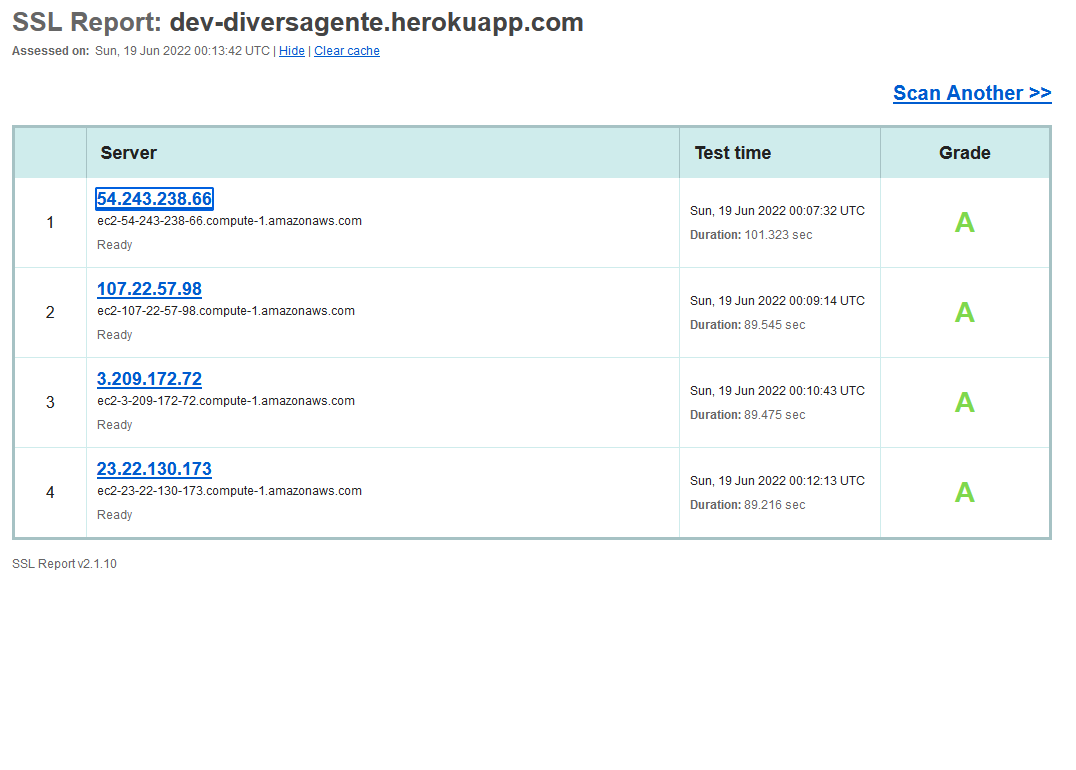
\includegraphics[width=1\textwidth]{anexos/SSLMetrica.png}
	\fonte{Fonte: Equipe diversaGente} 
\end{figure}
